\documentclass[10pt,letterpaper]{article}


\usepackage[latin1]{inputenc}
\usepackage{amsmath}
\usepackage{amsfonts}
\usepackage{amssymb}
\usepackage{graphicx}
\usepackage{fouridx}
\author{James Goppert}
\title{OpenFDM}

\newcommand{\ddt}[1]{\fourIdx{#1}{}{}{}{\frac{d}{dt}}}
\newcommand{\vect}[3]{\fourIdx{}{}{#3}{#2}{\mathbf{#1}}}
\newcommand{\vectDot}[3]{\fourIdx{}{}{#3}{#2}{\dot{\mathbf{#1}}}}
\newcommand{\cross}[0]{\times}

\newcommand{\wie}[0]{\vect{\omega}{ie}{}}
\newcommand{\wien}[0]{\vect{\omega}{ie}{n}}
\newcommand{\wiee}[0]{\vect{\omega}{ie}{e}}
\newcommand{\dwien}[0]{\vectDot{\omega}{ie}{n}}
\newcommand{\dwiee}[0]{\vectDot{\omega}{ie}{e}}
\newcommand{\wen}[0]{\vect{\omega}{en}{}}
\newcommand{\wenn}[0]{\vect{\omega}{en}{n}}
\newcommand{\ve}[0]{\vect{v}{e}{}}
\newcommand{\ven}[0]{\vect{v}{e}{n}}
\newcommand{\dven}[0]{\vectDot{v}{e}{n}}
\newcommand{\vi}[0]{\vect{v}{i}{}}
\newcommand{\ai}[0]{\vect{a}{i}{}}
\newcommand{\aib}[0]{\vect{a}{i}{b}}
\newcommand{\rv}[0]{\vect{r}{}{}}
\newcommand{\rve}[0]{\vect{r}{}{e}}
\newcommand{\rvn}[0]{\vect{r}{}{n}}
\newcommand{\C}[2]{\fourIdx{}{}{#1}{#2}{\mathbf{C}}}
\newcommand{\sumF}[0]{\vect{F}{}{}}
\newcommand{\sumFb}[0]{\vect{F}{b}{}}

\begin{document}

\maketitle
\newpage

\section*{Notation}
\begin{itemize}
\item $\vect{v}{r}{w}$ : A vector $\vect{v}{}{}$ with components expressed in frame $w$ and any derivatives are taken with respect to frame $r$.
\item $\ddt{i}\vect{v}{}{}$ : The derivative with respect to frame $i$ of vector $\vect{v}{}{}$.
\end{itemize}

\section{Equations of Motion}

\subsection{Translational Dynamics}

We start with Newton's second law and solve for the inertial acceleration $\ai$. Note that we allow for variable mass. This is important for rocket dynamics.

\begin{align}
\sumF &= \ddt{i} \left(m \vi \right) \notag \\
&= \dot{m} \vi + m \ai \notag \\
\ai &= \sumF/m - \left(\dot{m}/m\right) \vi
\label{eq:trans_dyn}
\end{align}

\subsection{Translational Kinematics}

\begin{figure}[ht!]
\center
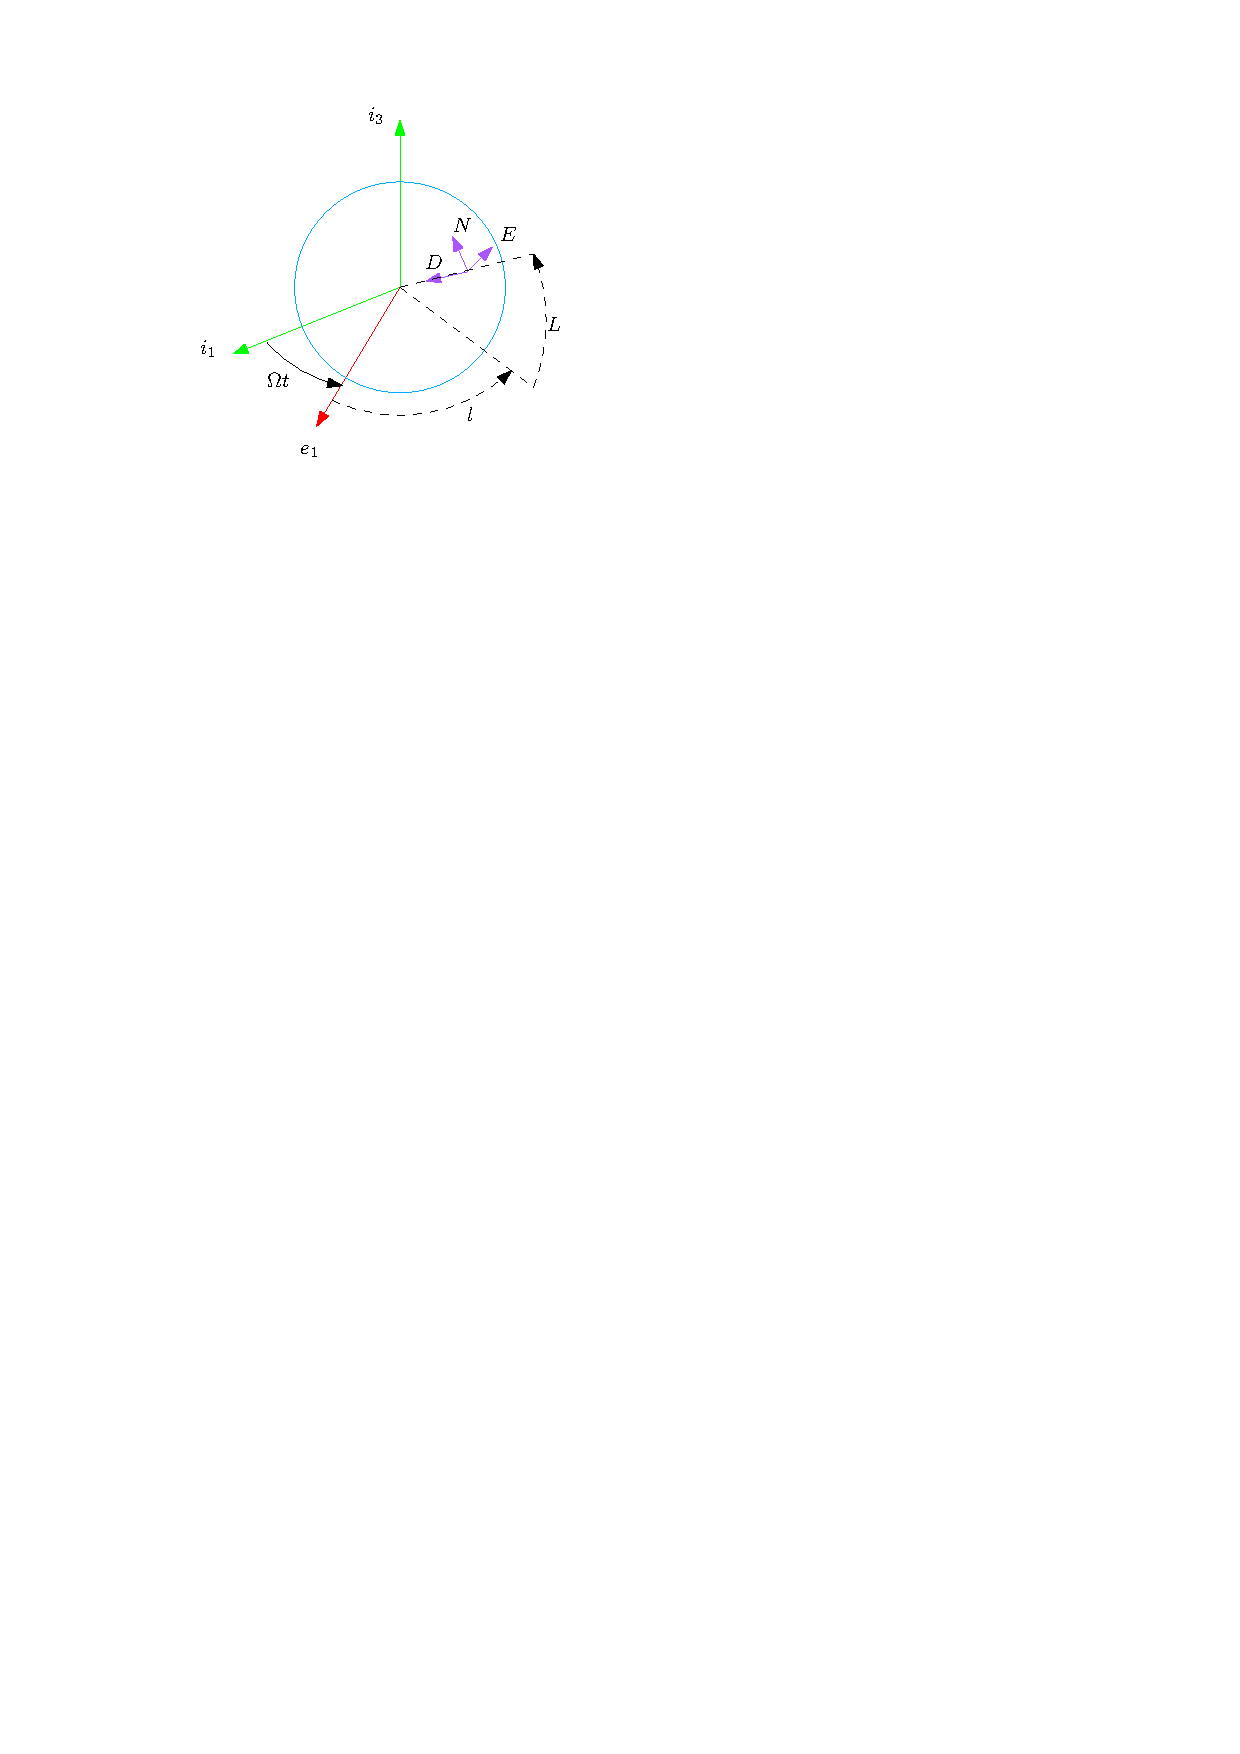
\includegraphics[scale=1]{fig/frames.pdf} 
\caption{Frame definitions}
\end{figure}

Frames
\begin{itemize}
\item i -- inertial frame (celestially fixed)
\item e -- reference frame (planet)
\item n -- navigation frame (local-tangent-plane)
\item b -- body frame (fixed in aircraft)
\end{itemize}

Through application of the basic kinematic equation we obtain an expression relating the velocity in the inertial frame $i$, to the velocity in the reference frame $e$. We let $\ve \equiv \ddt{e} \rv$ and
$\vi \equiv \ddt{i} \rv$:
\begin{align}
\ddt{i}\rv &= \ddt{e} \rv + \wie \cross \rv \notag \\
\vi &= \ve + \wie \cross \rv
\label{eq:ve}
\end{align}

We differentiate in the inertial frame and let $\ai \equiv \ddt{i} \vi$:
\begin{align}
\ddt{i} \ve &= \ddt{i} \vi - \ddt{i} \left( \wie \cross \rv \right) \notag \\
&= \ai - \ddt{e} \left( \wie \right) \cross \rv - \wie \cross \ve -  \wie \cross  \wie \cross \rv
\label{eq:ddt_i_ve}
\end{align}

We differentiate in the navigation frame:
\begin{align}
\ddt{n} \ve &= \ddt{i} \ve - \left(\wie + \wen \right) \cross \ve 
\label{eq:ddt_n_ve}
\end{align}

Combining Eq~\ref{eq:ddt_i_ve} and Eq~\ref{eq:ddt_n_ve}:
\begin{align}
\ddt{n} \ve &=  \ai - \ddt{e} \left( \wie \right) \cross \rv - \wie \cross \ve -  \wie \cross  \wie \cross \rv - \left(\wie + \wen \right) \cross \ve \notag \\
&= \ai - \ddt{e} \left( \wie \right) \cross \rv - \left(2 \wie + \wen \right) \cross \ve -  \wie \cross  \wie \cross \rv
\label{trans_kin}
\end{align}

Combining Eq~\ref{eq:trans_dyn} and \ref{trans_kin}:
\begin{align}
\begin{split}
\ddt{n} \ve &= \sumF/m - \left(\dot{m}/m\right) \left(\ve + \wie \cross \rv\right) - \ddt{e} \left( \wie \right) \cross \rv\\
& - \left(2 \wie + \wen \right) \cross \ve -  \wie \cross  \wie \cross \rv
\end{split}
\label{trans_eom}
\end{align}

We resolve the above equation in navigation frame, where $\C{n}{b}$ is a direction cosine matrix rotating from the body to the navigation frame, and $\C{n}{e}$ is a direction cosine matrix rotating from the reference to the navigation frame. First we resolve several angular velocities and the position vector in the navigation frame. Typically $\wiee =  \left[ 0, 0, \Omega \right]^T$ and $\dwiee =  \left[ 0, 0, \dot{\Omega} \right]^T$ when navigating on the surface of a planet. It is also typically assumed that $\dot{\Omega}=0$. The position vector in the reference frame of the planet is $\rve$. The contribution of the translational velocity in the reference frame to the angular velocity of the navigation frame is taken into about by the transport rate $\wenn$. $R_N$ is the meridian radius of curvature, and $R_E$ is the transverse radius of curvature.

\begin{align*}
\wien &= \C{n}{e} \wiee \\
\dwien &= \C{n}{e} \dwiee \\
\rvn &= \C{n}{e} \rve \\
R_N &= \frac{R\left(1-e^2\right)}{\left(1-e^2 \sin^2 L \right)^{3/2}} \\
R_E &= \frac{R}{\left(1-e^2 \sin^2 L \right)^{1/2}} \\
\wenn &= \left[ \frac{v_E}{R_E + h},  \frac{-v_N}{R_N + h},  \frac{-v_E \ \tan L}{R_N + h} \right]^T
\end{align*}

Then we solve for the translational equations of motion.
\begin{align}
\dven &= \C{n}{b}\sumFb/m - \left(\dot{m}/m\right) \left(\ven + \wien \cross \rvn  \right) - \dwien \cross \rvn \notag \\
& -  \left(2 \wien + \wenn \right) \cross \ven - \left( \wien \cross  \wien \cross \rvn \right) \\
\end{align}

If the position is maintained in geodetic coordinates, the derivative of these coordinates is given by:
\begin{align}
\dot{L} &= \frac{v_N}{R_N + h} \\
\dot{l} &= \frac{v_E}{\cos L \left( R_E + h \right) } \\
\dot{h} &= - v_D
\end{align}

\begin{table} [ht!]
\begin{tabular}{|l|c|c|}
\hline 
Length of semi-major axis & R & 6378137.0 m \\ 
\hline 
Major eccentricity of ellipsoid & e & 0.0818191908426 \\ 
\hline 
Earth's rotational rate & $\Omega$ & $7.292115 \times 10^{-5}$ rad/s \\ 
\hline 
\end{tabular} 
\caption{The WGS-84 model.}
\end{table}

\section{Attitude Equations of Motion}


\section{Rigid Body Connector}

\end{document}